\SourcePage{511}{514}
\section{Classification of molecular terms}

The molecular wave function is a product of an electronic wave function, a wave function for the vibrational motion of the nuclei, and a rotational wave function. The classification and symmetry types of these factors separately have already been discussed. It remains to classify molecular terms as a whole, that is, to determine the possible symmetries of the complete wave function.

Plainly, specifying the symmetry of all three factors under particular operations also fixes the symmetry of their product under those operations. A complete characterization of the state's symmetry must further specify how the total wave function behaves when the coordinates of every particle in the molecule, electrons and nuclei alike, are inverted simultaneously. A state is called \emph{negative} or \emph{positive} according as its wave function changes sign or remains unchanged under this operation\footnote{Following customary usage, we employ the same unsatisfactory terminology as for diatomic molecules (see \S~86).}.

It must be remembered, however, that inversion parity is meaningful only for molecules without stereoisomers. Stereoisomerism means that inversion takes a molecule into a configuration that cannot be brought into coincidence with the initial one by any spatial rotation (the ``right'' and ``left'' forms of a substance)\footnote{Stereoisomerism is possible only if the molecule has no symmetry element involving reflection: no inversion centre, symmetry plane, or rotation--reflection axis.}. When stereoisomerism is present, wave functions related by inversion therefore belong in essence to different molecules and there is no meaning in comparing them\footnote{Strictly, quantum mechanics always gives a nonzero probability for passage from one form to the other. This probability, involving passage of the nuclei through a barrier, is exceedingly small.}.

We saw in \S~86 that nuclear spin has an important indirect effect on the term scheme of a diatomic molecule: it fixes degeneracy multiplicities and can in some cases exclude levels of particular symmetry altogether. The same phenomenon occurs in polyatomic molecules. Its analysis is appreciably more complicated there, however, and requires group-theoretical methods in each particular case.

The method is based on the following idea. Besides the coordinate part

\SourcePage{512}{515}
(the only part considered thus far), the complete wave function must contain a spin factor depending on the projections of all nuclear spins upon some chosen direction in space. The projection $\sigma$ of a nuclear spin takes $2i+1$ values, where $i$ is the nuclear spin. Allowing all $\sigma_1,\sigma_2,\ldots,\sigma_N$, with $N$ the number of atoms in the molecule, to assume every possible value gives $(2i_1+1)(2i_2+1)\ldots(2i_N+1)$ distinct values of the spin factor. A symmetry operation interchanges certain nuclei of the same kind. If the spin values are imagined to remain fixed in position, the operation is equivalent to permuting those values among the nuclei. The different spin factors consequently transform into one another and thus realize a representation of the molecular symmetry group, generally a reducible one. Decomposition into irreducible parts then gives the possible symmetry types of the spin wave function.

A general formula for the characters $\chi_{\mathrm{sp}}(G)$ of the representation realized by the spin factors is immediate. Under an operation, the only unchanged spin factors are those for which nuclei being interchanged have the same $\sigma_a$; otherwise one spin factor is carried into another and contributes nothing to the character. Since $\sigma_a$ has $2i_a+1$ possible values, we obtain
\begin{equation}
 \chi_{\mathrm{sp}}(G)=\prod(2i_a+1), \tag{105.1}
\end{equation}
where the product extends over the sets of atoms permuted among themselves by the operation $G$, with one factor for each set.

Our main concern, however, is not the symmetry of the spin function but that of the coordinate wave function; here symmetry refers to permutations of the nuclear coordinates with the electron coordinates held fixed. These two symmetries are directly connected. Under interchange of any pair of nuclei obeying Bose or Fermi statistics, respectively, the complete wave function must remain unchanged or reverse sign. In other words, it is multiplied by $(-1)^{2i}$, where $i$ is the spin of the exchanged nuclei. Introducing this factor into the characters (105.1), we obtain the character system $\chi(G)$ for a representation containing all the irreducible representations according to which coordinate wave functions can transform:
\begin{equation}
 \chi(G)=\prod(2i_a+1)(-1)^{2i_a(n_a-1)}. \tag{105.2}
\end{equation}

\SourcePage{513}{516}
Here $n_a$ is the number of nuclei in each set permuted among itself by the given operation. Decomposing this representation into irreducible components yields the possible symmetry types of a molecule's coordinate wave functions together with the degeneracy multiplicities of the corresponding energy levels; here and below, the degeneracy is with respect to the different spin states of the nuclear system\footnote{In this connection the degeneracy multiplicity of a level is often called its nuclear statistical weight (compare the note on p.~407).}.

Each state-symmetry type is associated with definite values of the resultant spins of the groups of equivalent nuclei in the molecule, meaning groups whose members are interchanged by molecular symmetry operations. The association is not one-to-one: in general, a given state-symmetry type can occur with several values of the spins of the equivalent-nucleus groups. Group-theoretical methods can likewise establish this association in each particular case.

As an example, consider ethylene, ${}^{12}\mathrm C_2{}^1\mathrm H_4$, an asymmetric-top molecule (Fig.~43g, symmetry group $D_{2h}$). A superscript on a chemical symbol specifies the isotope of the nucleus; this information is needed because different isotopes may have different nuclear spins. Here the spin of the ${}^1\mathrm H$ nucleus is one half, whereas the ${}^{12}\mathrm C$ nucleus has no spin. Only the hydrogen atoms need therefore be considered.

Choose the coordinate system as in Fig.~43g, with the $z$ axis normal to the molecular plane and the $x$ axis along the molecular axis. Reflection in the plane $\sigma(xy)$ leaves every atom fixed, while the remaining reflections and rotations interchange the hydrogen atoms pairwise. Formula (105.2) gives the following characters:
\[
\begin{array}{c|cccccccc}
 &E&\sigma(xy)&\sigma(xz)&\sigma(yz)&I&C_2(z)&C_2(y)&C_2(x)\\ \hline
 &16&16&4&4&4&4&4&4
\end{array}
\]
On decomposition, this representation contains the following irreducible representations of $D_{2h}$: $7A_g$, $3B_{1g}$, $3B_{2u}$, and $3B_{3u}$. The numeral gives the multiplicity of the corresponding irreducible representation in the reducible representation; these numbers are precisely the nuclear statistical weights of levels of the corresponding symmetries\footnote{For the relation between state symmetry and the resultant spin of the four H nuclei in ethylene, see Problem 1.}.

\SourcePage{514}{517}
The resulting classification of ethylene states concerns the symmetry of the complete coordinate wave function, which includes electronic, vibrational, and rotational parts. It is usually useful to view the result in another way. Once the possible symmetries of the complete wave function are known, one can directly determine which rotational levels are allowed, and with what statistical weights, for a specified electronic and vibrational state.

For example, consider the rotational structure of the lowest vibrational level, with no vibrations excited, of the normal electronic term. We take the normal state's electronic wave function to be totally symmetric, as is true for practically all polyatomic molecules. The symmetry of the complete wave function under rotations about symmetry axes then coincides with that of the rotational wave function. Comparison with the result above shows that in ethylene the rotational levels of types $A$ and $B_1$ (see \S~103) are positive and have statistical weights 7 and 3, whereas levels of types $B_2$ and $B_3$ are negative and have statistical weight 3.

As in diatomic molecules (see the end of \S~86), transitions between ethylene states of different nuclear symmetry are practically absent because the nuclear-spin interaction with the electrons is extremely weak. Molecules in these states therefore behave as distinct forms of the substance; ethylene ${}^{12}\mathrm C_2{}^1\mathrm H_4$ has four such forms, with nuclear statistical weights 7, 3, 3, and 3. This conclusion relies essentially on the states of different symmetry belonging to different energy levels, whose separations are large compared with the energy of the nuclear-spin interaction. It is consequently inapplicable to molecules in which states of different nuclear symmetry belong to one and the same degenerate energy level.

Now consider ammonia ${}^{14}\mathrm N{}^1\mathrm H_3$, a symmetric-top molecule (Fig.~41, symmetry group $C_{3v}$). The spin of ${}^{14}\mathrm N$ is 1 and that of ${}^1\mathrm H$ is one half. Formula (105.2) gives the characters of the relevant representation of $C_{3v}$:
\[
\begin{array}{c|ccc}&E&2C_3&3\sigma_v\\\hline&24&6&-12\end{array}
\]
It contains the following irreducible representations of the group

\SourcePage{515}{518}
$C_{3v}$: $12A_2$ and $6E$. Two types of level are therefore possible, with nuclear statistical weights 12 and 6\footnote{Terms of symmetry $A_2$ correspond to a resultant hydrogen-nucleus spin of $3/2$, and terms $E$ to spin $1/2$.

The occurrence of the two-dimensional representation $E$ among the irreducible representations does not imply an additional degeneracy of the molecular energy levels. It is an instance of the permutation degeneracy discussed in \S~63.}.

For fixed $J$, the rotational levels of a symmetric top are classified by the quantum number $k$. As in the preceding example, consider the rotational structure of the normal electronic and vibrational states of $\mathrm{NH}_3$, taking both wave functions to be totally symmetric. In determining the rotational wave function's symmetry, only its behaviour under rotations about axes has meaning. We therefore replace each symmetry plane by a second-order symmetry axis normal to it; reflection in a plane is equivalent to rotation about such an axis followed by inversion. Thus $C_{3v}$ is replaced here by the isomorphic point group $D_3$.

Under a $C_3$ rotation about the vertical third-order axis, the rotational wave functions with $k=\pm|k|$ acquire the factors $e^{\pm2\pi i|k|/3}$; a $U_2$ rotation about a horizontal second-order axis interchanges them. They therefore realize a two-dimensional representation of $D_3$. If $|k|$ is not divisible by three, this is the irreducible representation $E$. The representation of $C_{3v}$ belonging to the complete wave function is obtained by multiplying the character $\chi(U_2)$ by $+1$ or $-1$ according as the term is positive or negative. Since $\chi(U_2)=0$ in $E$, both choices again yield $E$, now as a representation of $C_{3v}$ rather than $D_3$. The preceding results therefore show that for $|k|$ not divisible by three, both positive and negative levels are possible, with nuclear statistical weight 6; the complete coordinate wave function has symmetry $E$. For nonzero $|k|$ divisible by three, the rotational functions realize the representation of $D_3$ whose characters are
\[
\begin{array}{c|ccc}&E&2C_3&3U_2\\\hline&2&2&0\end{array}.
\]

\SourcePage{516}{519}
This representation is reducible and decomposes into $A_1$ and $A_2$. For the complete wave function to belong to $A_2$ of $C_{3v}$, the $A_1$ rotational level must be negative and the $A_2$ level positive. Hence, when nonzero $|k|$ is divisible by three, both positive and negative levels occur with nuclear statistical weight 12; these are levels of type $A_2$.

For $k=0$ there is only one rotational function. It realizes a representation with characters\footnote{Under rotation through an angle $\pi$, an angular-momentum eigenfunction with magnitude $J$ and zero projection is multiplied by $(-1)^J$.}
\[
\begin{array}{c|ccc}&E&2C_3&3U_2\\\hline&1&1&(-1)^J\end{array}.
\]
For the complete wave function to have symmetry $A_2$, its inversion behaviour must consequently be specified by the factor $-(-1)^J$. Thus, at $k=0$, levels with even (odd) $J$ can only be negative (positive); in both cases the statistical weight is 12, and the levels are of type $A_2$.

Combining these results gives the following table of states allowed at various $k$ for the normal electronic and vibrational term of ${}^{14}\mathrm N{}^1\mathrm H_3$; $+$ and $-$ denote positive and negative states:
\[
\begin{array}{l|cc}
 &(+)&(-)\\\hline
|k|\text{ not divisible by three}&6E&6E\\
|k|\text{ divisible by three}&12A_2&12A_2\\
k=0,\ J\text{ even}&-&12A_2\\
k=0,\ J\text{ odd}&12A_2&-
\end{array}
\]
For specified $J$ and $k$, the energy levels of $\mathrm{NH}_3$ are generally degenerate (see also the table for $\mathrm{ND}_3$ in Problem 3). This degeneracy is partly lifted by a distinctive effect associated with the shallow pyramidal shape of ammonia and the low mass of the hydrogen atoms. A comparatively small vertical displacement of the atoms permits passage between two configurations that are mirror images in a plane parallel to the base of the pyramid (Fig.~44). These transitions split the levels,

\SourcePage{517}{520}
separating the positive from the negative levels; the effect is analogous to the one-dimensional case considered in Problem 3 of \S~50.

\setcounter{figure}{43}
\begin{figure}[ht]
\centering
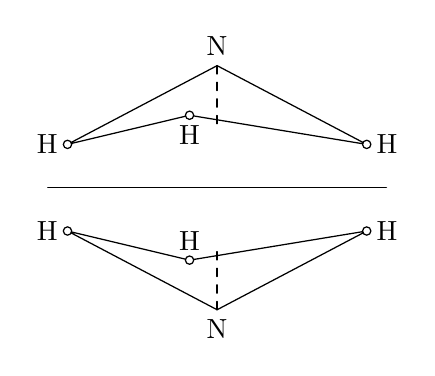
\begin{tikzpicture}[x=1cm,y=1cm,line width=.45pt,line cap=round]
  \draw (-2.15,0)--(2.15,0);
  \coordinate (Lt) at (-1.9,.55); \coordinate (Rt) at (1.9,.55);
  \coordinate (Nt) at (0,1.55); \coordinate (Ct) at (-.35,.92);
  \draw (Lt)--(Nt)--(Rt)--(Ct)--cycle;
  \draw[dashed] (Nt)--(0,.75);
  \filldraw[fill=white] (Lt) circle (1.5pt) (Rt) circle (1.5pt) (Ct) circle (1.5pt);
  \node[left] at (Lt) {H}; \node[right] at (Rt) {H}; \node[above] at (Nt) {N}; \node[below] at (Ct) {H};
  \coordinate (Lb) at (-1.9,-.55); \coordinate (Rb) at (1.9,-.55);
  \coordinate (Nb) at (0,-1.55); \coordinate (Cb) at (-.35,-.92);
  \draw (Lb)--(Nb)--(Rb)--(Cb)--cycle;
  \draw[dashed] (Nb)--(0,-.75);
  \filldraw[fill=white] (Lb) circle (1.5pt) (Rb) circle (1.5pt) (Cb) circle (1.5pt);
  \node[left] at (Lb) {H}; \node[right] at (Rb) {H}; \node[below] at (Nb) {N}; \node[above] at (Cb) {H};
\end{tikzpicture}
\caption{}
\end{figure}

The splitting is proportional to the probability for the atoms to pass through the ``potential barrier'' separating the two molecular configurations. Owing to the properties just described, this probability is comparatively large in ammonia, but the splitting nevertheless remains small, $1\cdot10^{-4}$ eV. A spherical-top molecule is treated in Problem 5 of this section.

\subsection*{Problems}

\ProblemHeading 1. Establish the relation between the symmetry of the states of ${}^{12}\mathrm C_2{}^1\mathrm H_4$ and the resultant spin of its hydrogen nuclei.

\SolutionHeading\footnote{For a solution method based on the theory of permutation groups, see the book by I.~G.~Kaplan cited on p.~291, Chapter VI, \S~2.} The resultant spin of four ${}^1\mathrm H$ nuclei can take the values $I=2,1,0$, while its projection $M_I$ ranges from 2 to $-2$. Beginning with the largest value, consider the representations realized by the spin factors belonging to each separate value of $M_I$.

For $M_I=2$ there is just one spin factor, in which every nucleus has spin projection $+1/2$. For $M_I=1$ there are four distinct spin factors, distinguished by which of the four nuclei is assigned spin projection $-1/2$. Finally, $M_I=0$ is realized by six spin factors, according to which pair of nuclei is assigned projection $-1/2$. The characters of the three corresponding representations are
\[
\begin{array}{c|cccccccc}
 &E&\sigma(xy)&\sigma(xz)&\sigma(yz)&I&C_2(z)&C_2(y)&C_2(x)\\\hline
M_I=2&1&1&1&1&1&1&1&1\\
M_I=1&4&4&0&0&0&0&0&0\\
M_I=0&6&6&2&2&2&2&2&2
\end{array}
\]
The first is the identity representation $A_g$. Since $M_I=2$ is possible only for $I=2$, a state of symmetry $A_g$ corresponds to spin $I=2$.

The value $M_I=1$ is possible for both $I=1$ and $I=2$. Accordingly subtracting the first representation from the second and decomposing the result into irreducible components, we find that spin $I=1$ corresponds to states $B_{1g}$, $B_{2u}$, and $B_{3u}$.

Finally, $M_I=0$ occurs whenever $M_I=1$ is possible and also for $I=0$. Subtracting the second representation from the third accordingly gives two $A_g$ states corresponding to spin $I=0$.

\ProblemHeading 2. Determine the symmetry types of the complete coordinate wave functions and the statistical weights of the corresponding levels for the molecules

\SourcePage{518}{521}
${}^{12}\mathrm C_2{}^2\mathrm H_4$, ${}^{13}\mathrm C_2{}^1\mathrm H_4$, and ${}^{14}\mathrm N_2{}^{16}\mathrm O_4$ (all have the same shape); the spins are $i({}^2\mathrm H)=1$, $i({}^{13}\mathrm C)=1/2$, and $i({}^{14}\mathrm N)=1$.

\SolutionHeading By the same method used in the text for ${}^{12}\mathrm C_2{}^1\mathrm H_4$, we obtain the following states; the coordinate axes are chosen as in the text:
\[
\begin{array}{c|c|c}
\text{Molecule}&(+)&(-)\\\hline
{}^{12}\mathrm C_2{}^2\mathrm H_4&27A_g,\ 18B_{1g}&18B_{2u},\ 18B_{3u}\\
{}^{13}\mathrm C_2{}^1\mathrm H_4&16A_g,\ 12B_{1g}&12B_{2u},\ 24B_{2u}\\
{}^{14}\mathrm N_2{}^{16}\mathrm O_4&6A_g&3B_{3u}
\end{array}
\]

\ProblemHeading 3. Do the same for ${}^{14}\mathrm N{}^2\mathrm H_3$.

\SolutionHeading As for ${}^{14}\mathrm N{}^1\mathrm H_3$ in the text, we find the states $30A_1$, $3A_2$, and $24E$. For the normal electronic and vibrational term, the following states are possible at different values of $k$:
\[
\begin{array}{l|cc}&(+)&(-)\\\hline
|k|\text{ not divisible by three}&24E&24E\\
|k|\text{ divisible by three}&30A_1,3A_2&30A_1,3A_2\\
k=0,\ J\text{ even}&30A_1&3A_2\\
k=0,\ J\text{ odd}&3A_2&30A_1
\end{array}
\]

\ProblemHeading 4. Do the same for ${}^{12}\mathrm C_2{}^1\mathrm H_6$ (see Fig.~43e; symmetry $D_{3d}$).

\SolutionHeading The possible state types are $7A_{1g}$, $1A_{1u}$, $3A_{2g}$, $13A_{2u}$, $9E_g$, and $11E_u$.

For the normal electronic and vibrational term the states are
\[
\begin{array}{l|cc}&(+)&(-)\\\hline
|k|\text{ not divisible by three}&9E_g&11E_u\\
|k|\text{ divisible by three}&7A_{1g},3A_{2g}&1A_{1u},13A_{2u}\\
k=0,\ J\text{ even}&7A_{1g}&1A_{1u}\\
k=0,\ J\text{ odd}&3A_{2g}&13A_{2u}
\end{array}
\]

\ProblemHeading 5. Do the same for methane ${}^{12}\mathrm C{}^1\mathrm H_4$, with the H atoms at the vertices and the C atom at the centre of a tetrahedron.

\SolutionHeading The molecule is a spherical top of symmetry $T_d$. The same method gives possible states of types $5A_2$, $1E$, and $3F_1$, corresponding respectively to total molecular spin 2, 0, and 1. Rotational states of a spherical top are classified by the total angular momentum $J$. The $2J+1$ rotational functions belonging to a specified $J$ realize a $(2J+1)$-dimensional representation of the group $O$. This group is isomorphic to $T_d$ and is obtained from it

\SourcePage{519}{522}
by replacing every symmetry plane with the perpendicular second-order axis. The characters of this representation are given by formula (98.3). For example, $J=3$ gives the representation with characters
\[
\begin{array}{c|ccccc}&E&8C_3&6C_2&6C_4&3C_4^2\\\hline&7&1&-1&-1&-1\end{array}.
\]
It contains the following irreducible representations of $O$: $A_2$, $F_1$, and $F_2$. Returning to the rotational structure of the normal electronic and vibrational term, we infer that at $J=3$ states whose complete wave function has symmetry $A_2$ can only be positive, whereas the $F_1$ states may be either positive or negative. For the first few values of $J$, the states obtained in this way, with their nuclear statistical weights, are
\[
\begin{array}{c|cc}&(+)&(-)\\\hline
J=0&-&5A_2\\
J=1&3F_1&-\\
J=2&1E&1E,3F_1\\
J=3&5A_2,3F_1&3F_1\\
J=4&1E,3F_1&5A_2,1E,3F_1
\end{array}
\]
